% Options for packages loaded elsewhere
% Options for packages loaded elsewhere
\PassOptionsToPackage{unicode}{hyperref}
\PassOptionsToPackage{hyphens}{url}
\PassOptionsToPackage{dvipsnames,svgnames,x11names}{xcolor}
%
\documentclass[
  letterpaper,
  DIV=11,
  numbers=noendperiod]{scrreprt}
\usepackage{xcolor}
\usepackage{amsmath,amssymb}
\setcounter{secnumdepth}{5}
\usepackage{iftex}
\ifPDFTeX
  \usepackage[T1]{fontenc}
  \usepackage[utf8]{inputenc}
  \usepackage{textcomp} % provide euro and other symbols
\else % if luatex or xetex
  \usepackage{unicode-math} % this also loads fontspec
  \defaultfontfeatures{Scale=MatchLowercase}
  \defaultfontfeatures[\rmfamily]{Ligatures=TeX,Scale=1}
\fi
\usepackage{lmodern}
\ifPDFTeX\else
  % xetex/luatex font selection
\fi
% Use upquote if available, for straight quotes in verbatim environments
\IfFileExists{upquote.sty}{\usepackage{upquote}}{}
\IfFileExists{microtype.sty}{% use microtype if available
  \usepackage[]{microtype}
  \UseMicrotypeSet[protrusion]{basicmath} % disable protrusion for tt fonts
}{}
\makeatletter
\@ifundefined{KOMAClassName}{% if non-KOMA class
  \IfFileExists{parskip.sty}{%
    \usepackage{parskip}
  }{% else
    \setlength{\parindent}{0pt}
    \setlength{\parskip}{6pt plus 2pt minus 1pt}}
}{% if KOMA class
  \KOMAoptions{parskip=half}}
\makeatother
% Make \paragraph and \subparagraph free-standing
\makeatletter
\ifx\paragraph\undefined\else
  \let\oldparagraph\paragraph
  \renewcommand{\paragraph}{
    \@ifstar
      \xxxParagraphStar
      \xxxParagraphNoStar
  }
  \newcommand{\xxxParagraphStar}[1]{\oldparagraph*{#1}\mbox{}}
  \newcommand{\xxxParagraphNoStar}[1]{\oldparagraph{#1}\mbox{}}
\fi
\ifx\subparagraph\undefined\else
  \let\oldsubparagraph\subparagraph
  \renewcommand{\subparagraph}{
    \@ifstar
      \xxxSubParagraphStar
      \xxxSubParagraphNoStar
  }
  \newcommand{\xxxSubParagraphStar}[1]{\oldsubparagraph*{#1}\mbox{}}
  \newcommand{\xxxSubParagraphNoStar}[1]{\oldsubparagraph{#1}\mbox{}}
\fi
\makeatother

\usepackage{color}
\usepackage{fancyvrb}
\newcommand{\VerbBar}{|}
\newcommand{\VERB}{\Verb[commandchars=\\\{\}]}
\DefineVerbatimEnvironment{Highlighting}{Verbatim}{commandchars=\\\{\}}
% Add ',fontsize=\small' for more characters per line
\usepackage{framed}
\definecolor{shadecolor}{RGB}{241,243,245}
\newenvironment{Shaded}{\begin{snugshade}}{\end{snugshade}}
\newcommand{\AlertTok}[1]{\textcolor[rgb]{0.68,0.00,0.00}{#1}}
\newcommand{\AnnotationTok}[1]{\textcolor[rgb]{0.37,0.37,0.37}{#1}}
\newcommand{\AttributeTok}[1]{\textcolor[rgb]{0.40,0.45,0.13}{#1}}
\newcommand{\BaseNTok}[1]{\textcolor[rgb]{0.68,0.00,0.00}{#1}}
\newcommand{\BuiltInTok}[1]{\textcolor[rgb]{0.00,0.23,0.31}{#1}}
\newcommand{\CharTok}[1]{\textcolor[rgb]{0.13,0.47,0.30}{#1}}
\newcommand{\CommentTok}[1]{\textcolor[rgb]{0.37,0.37,0.37}{#1}}
\newcommand{\CommentVarTok}[1]{\textcolor[rgb]{0.37,0.37,0.37}{\textit{#1}}}
\newcommand{\ConstantTok}[1]{\textcolor[rgb]{0.56,0.35,0.01}{#1}}
\newcommand{\ControlFlowTok}[1]{\textcolor[rgb]{0.00,0.23,0.31}{\textbf{#1}}}
\newcommand{\DataTypeTok}[1]{\textcolor[rgb]{0.68,0.00,0.00}{#1}}
\newcommand{\DecValTok}[1]{\textcolor[rgb]{0.68,0.00,0.00}{#1}}
\newcommand{\DocumentationTok}[1]{\textcolor[rgb]{0.37,0.37,0.37}{\textit{#1}}}
\newcommand{\ErrorTok}[1]{\textcolor[rgb]{0.68,0.00,0.00}{#1}}
\newcommand{\ExtensionTok}[1]{\textcolor[rgb]{0.00,0.23,0.31}{#1}}
\newcommand{\FloatTok}[1]{\textcolor[rgb]{0.68,0.00,0.00}{#1}}
\newcommand{\FunctionTok}[1]{\textcolor[rgb]{0.28,0.35,0.67}{#1}}
\newcommand{\ImportTok}[1]{\textcolor[rgb]{0.00,0.46,0.62}{#1}}
\newcommand{\InformationTok}[1]{\textcolor[rgb]{0.37,0.37,0.37}{#1}}
\newcommand{\KeywordTok}[1]{\textcolor[rgb]{0.00,0.23,0.31}{\textbf{#1}}}
\newcommand{\NormalTok}[1]{\textcolor[rgb]{0.00,0.23,0.31}{#1}}
\newcommand{\OperatorTok}[1]{\textcolor[rgb]{0.37,0.37,0.37}{#1}}
\newcommand{\OtherTok}[1]{\textcolor[rgb]{0.00,0.23,0.31}{#1}}
\newcommand{\PreprocessorTok}[1]{\textcolor[rgb]{0.68,0.00,0.00}{#1}}
\newcommand{\RegionMarkerTok}[1]{\textcolor[rgb]{0.00,0.23,0.31}{#1}}
\newcommand{\SpecialCharTok}[1]{\textcolor[rgb]{0.37,0.37,0.37}{#1}}
\newcommand{\SpecialStringTok}[1]{\textcolor[rgb]{0.13,0.47,0.30}{#1}}
\newcommand{\StringTok}[1]{\textcolor[rgb]{0.13,0.47,0.30}{#1}}
\newcommand{\VariableTok}[1]{\textcolor[rgb]{0.07,0.07,0.07}{#1}}
\newcommand{\VerbatimStringTok}[1]{\textcolor[rgb]{0.13,0.47,0.30}{#1}}
\newcommand{\WarningTok}[1]{\textcolor[rgb]{0.37,0.37,0.37}{\textit{#1}}}

\usepackage{longtable,booktabs,array}
\usepackage{calc} % for calculating minipage widths
% Correct order of tables after \paragraph or \subparagraph
\usepackage{etoolbox}
\makeatletter
\patchcmd\longtable{\par}{\if@noskipsec\mbox{}\fi\par}{}{}
\makeatother
% Allow footnotes in longtable head/foot
\IfFileExists{footnotehyper.sty}{\usepackage{footnotehyper}}{\usepackage{footnote}}
\makesavenoteenv{longtable}
\usepackage{graphicx}
\makeatletter
\newsavebox\pandoc@box
\newcommand*\pandocbounded[1]{% scales image to fit in text height/width
  \sbox\pandoc@box{#1}%
  \Gscale@div\@tempa{\textheight}{\dimexpr\ht\pandoc@box+\dp\pandoc@box\relax}%
  \Gscale@div\@tempb{\linewidth}{\wd\pandoc@box}%
  \ifdim\@tempb\p@<\@tempa\p@\let\@tempa\@tempb\fi% select the smaller of both
  \ifdim\@tempa\p@<\p@\scalebox{\@tempa}{\usebox\pandoc@box}%
  \else\usebox{\pandoc@box}%
  \fi%
}
% Set default figure placement to htbp
\def\fps@figure{htbp}
\makeatother





\setlength{\emergencystretch}{3em} % prevent overfull lines

\providecommand{\tightlist}{%
  \setlength{\itemsep}{0pt}\setlength{\parskip}{0pt}}



 


\KOMAoption{captions}{tableheading}
\makeatletter
\@ifpackageloaded{bookmark}{}{\usepackage{bookmark}}
\makeatother
\makeatletter
\@ifpackageloaded{caption}{}{\usepackage{caption}}
\AtBeginDocument{%
\ifdefined\contentsname
  \renewcommand*\contentsname{Table of contents}
\else
  \newcommand\contentsname{Table of contents}
\fi
\ifdefined\listfigurename
  \renewcommand*\listfigurename{List of Figures}
\else
  \newcommand\listfigurename{List of Figures}
\fi
\ifdefined\listtablename
  \renewcommand*\listtablename{List of Tables}
\else
  \newcommand\listtablename{List of Tables}
\fi
\ifdefined\figurename
  \renewcommand*\figurename{Figure}
\else
  \newcommand\figurename{Figure}
\fi
\ifdefined\tablename
  \renewcommand*\tablename{Table}
\else
  \newcommand\tablename{Table}
\fi
}
\@ifpackageloaded{float}{}{\usepackage{float}}
\floatstyle{ruled}
\@ifundefined{c@chapter}{\newfloat{codelisting}{h}{lop}}{\newfloat{codelisting}{h}{lop}[chapter]}
\floatname{codelisting}{Listing}
\newcommand*\listoflistings{\listof{codelisting}{List of Listings}}
\makeatother
\makeatletter
\makeatother
\makeatletter
\@ifpackageloaded{caption}{}{\usepackage{caption}}
\@ifpackageloaded{subcaption}{}{\usepackage{subcaption}}
\makeatother
\usepackage{bookmark}
\IfFileExists{xurl.sty}{\usepackage{xurl}}{} % add URL line breaks if available
\urlstyle{same}
\hypersetup{
  pdftitle={Mi Tesis},
  pdfauthor={Tu Nombre},
  colorlinks=true,
  linkcolor={blue},
  filecolor={Maroon},
  citecolor={Blue},
  urlcolor={Blue},
  pdfcreator={LaTeX via pandoc}}


\title{Mi Tesis}
\author{Tu Nombre}
\date{2025-06-17}
\begin{document}
\maketitle

\renewcommand*\contentsname{Table of contents}
{
\hypersetup{linkcolor=}
\setcounter{tocdepth}{2}
\tableofcontents
}

\bookmarksetup{startatroot}

\chapter{thesis}\label{thesis}

\section{Quarto}\label{quarto}

Quarto enables you to weave together content and executable code into a
finished document. To learn more about Quarto see
\url{https://quarto.org}.

\bookmarksetup{startatroot}

\chapter{}\label{section}

\bookmarksetup{startatroot}

\chapter{}\label{section-1}

\bookmarksetup{startatroot}

\chapter{``Cálculo de distancia 3D de rutas geográficas usando datos
OSRM y
elevación''}\label{cuxe1lculo-de-distancia-3d-de-rutas-geogruxe1ficas-usando-datos-osrm-y-elevaciuxf3n}

Para estimar la longitud real de una carretera considerando las
variaciones de altitud del terreno, se utiliza una formulación basada en
la distancia geodésica entre puntos sucesivos de una ruta, combinada con
la diferencia de elevaciones. Esto permite obtener una distancia
tridimensional (3D) más realista, que considera tanto la curvatura
terrestre como los cambios topográficos.

Sea una ruta discretizada por \(N\) puntos geográficos con coordenadas:
\(P_i= (\phi_i, \lambda_i\)) para \(i=1, \cdots, N\) donde: \(\phi_i\)
es la latitud de punto \(i\) y \(\lambda_i\) es la longitud del punto
\(i\).

La distancia superficial (2D) entre dos puntos consecutivos se calcula
utilizando la fórmula de Vincenty o usando elipsoide WGS84 (World
Geodetic System 1984): \[
 d_i^{2D}= GeodInv(\phi_{i-1}, \lambda_{i-1}, \phi_i, \lambda_i)
 \]

\(d_i^{2D}\) es la distancia geodésica 2D entre los puntos \(P_{i-1}\) y
\(P_{i}\) calculada sobre la superficie de la Tierra.

Por otro lado para estimar la distancia real de una carretera
considerando la variaciones del terreno (elavación) se considera la ruta
de una secuencia de puntos geográficos \(P_i= (\phi_i, \lambda_i\)) y
\(h_i\) una elevación en metros sobre el nivel del mar en el punto
\(i\), extraÍda del mosaico ráster de altitudes mediente la
interpolacion espacial. La distancia entre dos puntos consecutivos se
calcula como: \[
d_i^{3D} = \sqrt{(d_i^{2D})^2+(\Delta h_i)^2}
\] siendo \(\Delta h_i= h_i-h_{i-1}\) es el cambio de altitud entre dos
puntos consecutivos.

La distancia total proyectada (2D) y la distancia real sobre el terreno
(3D) son \[
D^{(2D)}= \sum_{i=1}^{N-1} d_i^{(2D)}
\] \[
D^{(3D)}= \sum_{i=1}^{N-1} d_i^{(3D)}
\]

Este cálculo se implementó utilizando datos de OpenStreetMap y modelos
de elevación (DEM) rasterizados.

\bookmarksetup{startatroot}

\chapter{}\label{section-2}

\bookmarksetup{startatroot}

\chapter{Mapa con Folium}\label{mapa-con-folium}

\bookmarksetup{startatroot}

\chapter{Mapa interactivo con Folium}\label{mapa-interactivo-con-folium}

\begin{Shaded}
\begin{Highlighting}[]
\ImportTok{import}\NormalTok{ folium}

\CommentTok{\# Crear el mapa centrado en Tuxtla Gutiérrez}
\NormalTok{mapa }\OperatorTok{=}\NormalTok{ folium.Map(location}\OperatorTok{=}\NormalTok{[}\FloatTok{16.7529}\NormalTok{, }\OperatorTok{{-}}\FloatTok{93.1169}\NormalTok{], zoom\_start}\OperatorTok{=}\DecValTok{13}\NormalTok{)}

\CommentTok{\# Agregar un marcador}
\NormalTok{folium.Marker(}
\NormalTok{    [}\FloatTok{16.7529}\NormalTok{, }\OperatorTok{{-}}\FloatTok{93.1169}\NormalTok{],}
\NormalTok{    tooltip}\OperatorTok{=}\StringTok{"Tuxtla Gutiérrez"}\NormalTok{,}
\NormalTok{    popup}\OperatorTok{=}\StringTok{"Capital de Chiapas"}
\NormalTok{).add\_to(mapa)}

\CommentTok{\# Guardar el mapa como archivo HTML para Selenium}
\NormalTok{mapa.save(}\StringTok{"mapa\_folium.html"}\NormalTok{)}
\end{Highlighting}
\end{Shaded}

\begin{Shaded}
\begin{Highlighting}[]
\ImportTok{import}\NormalTok{ IPython}
\NormalTok{IPython.display.display(mapa)}
\end{Highlighting}
\end{Shaded}

\begin{verbatim}
<folium.folium.Map at 0x26d2814e510>
\end{verbatim}

\begin{Shaded}
\begin{Highlighting}[]
\CommentTok{\# Captura del mapa como imagen PNG para incluir en PDF}
\CommentTok{\# Captura del mapa como imagen PNG para incluir en PDF}
\ImportTok{import}\NormalTok{ os}
\ImportTok{from}\NormalTok{ selenium }\ImportTok{import}\NormalTok{ webdriver}
\ImportTok{from}\NormalTok{ selenium.webdriver.chrome.options }\ImportTok{import}\NormalTok{ Options}
\ImportTok{from}\NormalTok{ PIL }\ImportTok{import}\NormalTok{ Image}
\ImportTok{import}\NormalTok{ time}

\ControlFlowTok{if} \KeywordTok{not}\NormalTok{ os.path.exists(}\StringTok{"mapa\_folium.png"}\NormalTok{):}
\NormalTok{    options }\OperatorTok{=}\NormalTok{ Options()}
\NormalTok{    options.add\_argument(}\StringTok{\textquotesingle{}{-}{-}headless\textquotesingle{}}\NormalTok{)}
\NormalTok{    options.add\_argument(}\StringTok{\textquotesingle{}{-}{-}disable{-}gpu\textquotesingle{}}\NormalTok{)}
\NormalTok{    options.add\_argument(}\StringTok{\textquotesingle{}{-}{-}disable{-}dev{-}shm{-}usage\textquotesingle{}}\NormalTok{)}
\NormalTok{    options.add\_argument(}\StringTok{"{-}{-}window{-}size=800,600"}\NormalTok{)}

\NormalTok{    driver }\OperatorTok{=}\NormalTok{ webdriver.Chrome(options}\OperatorTok{=}\NormalTok{options)}

\NormalTok{    driver.get(}\StringTok{"file://"} \OperatorTok{+}\NormalTok{ os.path.abspath(}\StringTok{"mapa\_folium.html"}\NormalTok{))}
\NormalTok{    time.sleep(}\DecValTok{2}\NormalTok{)  }\CommentTok{\# Esperar a que cargue el mapa}

    \CommentTok{\# Forzar fondo blanco (evita fondo negro)}
\NormalTok{    driver.execute\_script(}\StringTok{"document.body.style.background = \textquotesingle{}white\textquotesingle{};"}\NormalTok{)}

    \CommentTok{\# Intentar capturar el contenedor del mapa directamente}
    \ControlFlowTok{try}\NormalTok{:}
\NormalTok{        map\_element }\OperatorTok{=}\NormalTok{ driver.find\_element(}\StringTok{"id"}\NormalTok{, }\StringTok{"map"}\NormalTok{)}
\NormalTok{        map\_element.screenshot(}\StringTok{"mapa\_folium.png"}\NormalTok{)}
    \ControlFlowTok{except}\NormalTok{:}
        \CommentTok{\# Si no encuentra el ID, captura toda la pantalla y recorta}
\NormalTok{        driver.save\_screenshot(}\StringTok{"mapa\_folium\_full.png"}\NormalTok{)}
\NormalTok{        img }\OperatorTok{=}\NormalTok{ Image.}\BuiltInTok{open}\NormalTok{(}\StringTok{"mapa\_folium\_full.png"}\NormalTok{)}
\NormalTok{        crop }\OperatorTok{=}\NormalTok{ img.crop((}\DecValTok{0}\NormalTok{, }\DecValTok{0}\NormalTok{, }\DecValTok{800}\NormalTok{, }\DecValTok{600}\NormalTok{))}
\NormalTok{        crop.save(}\StringTok{"mapa\_folium.png"}\NormalTok{)}

\NormalTok{    driver.quit()}
\end{Highlighting}
\end{Shaded}

\begin{figure}[H]

{\centering \pandocbounded{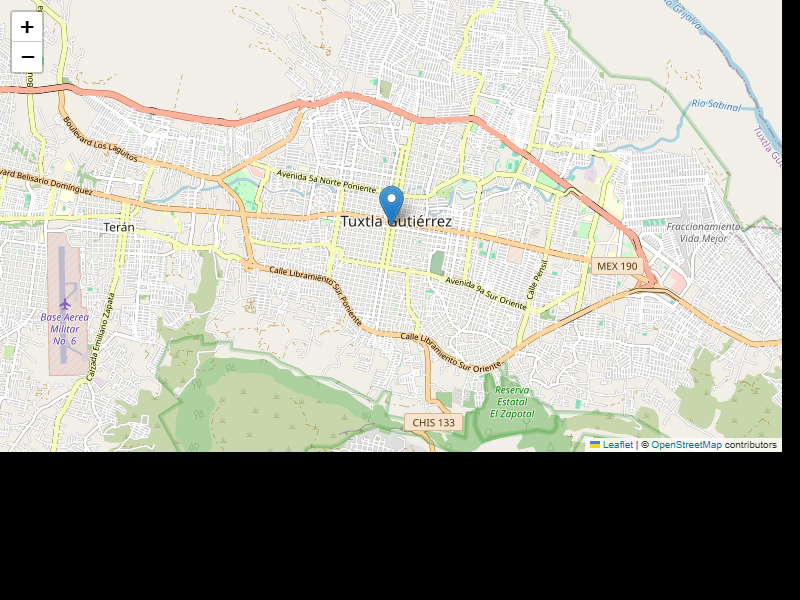
\includegraphics[keepaspectratio]{mapa_folium.png}}

}

\caption{Mapa generado con Folium}

\end{figure}%




\end{document}
